\documentclass[12pt, letterpaper]{article}
\usepackage[a4paper, margin=1in]{geometry}
\usepackage{graphicx}
\usepackage{float}
\graphicspath{{images/}}
\author{Joseph Yu}
\title{Lab 1: Spike Neural Networks}
\begin{document}
\maketitle
\setcounter{section}{4}
\subsection{Hyperparameter Tuning}
\begin{figure}[H]
    \centering
    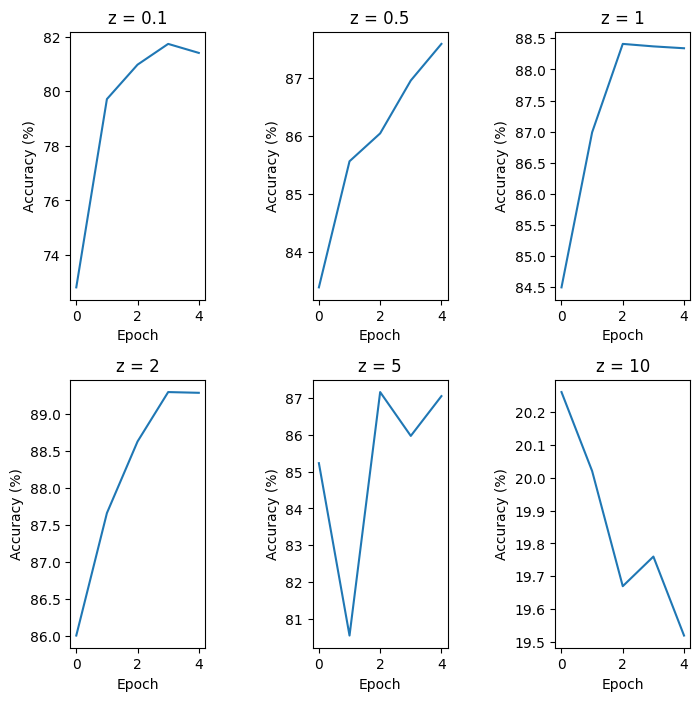
\includegraphics[width=0.75\textwidth]{z_parameter_tuning.png}
    \caption{Tuning $z$ hyperparameter}
    \label{fig:z_tuning}
\end{figure}
From the graphs of test accuracy with increasing $z$ values in Figure \ref{fig:z_tuning} we can see that the performance steadily improves up to $z = 2$ and then starts to decrease. At $z = 10$ the accuracy is below 20\% and additional training epochs does not show any improvement in the accuracy. This could be attributed to as z increases the fast Sigmoid function begins to approach the shape of a step function, which makes it difficult for the network to learn. since the derivative of the fast Sigmoid function for large $z$ is zero for most of the input range.

\begin{figure}[H]
    \centering
    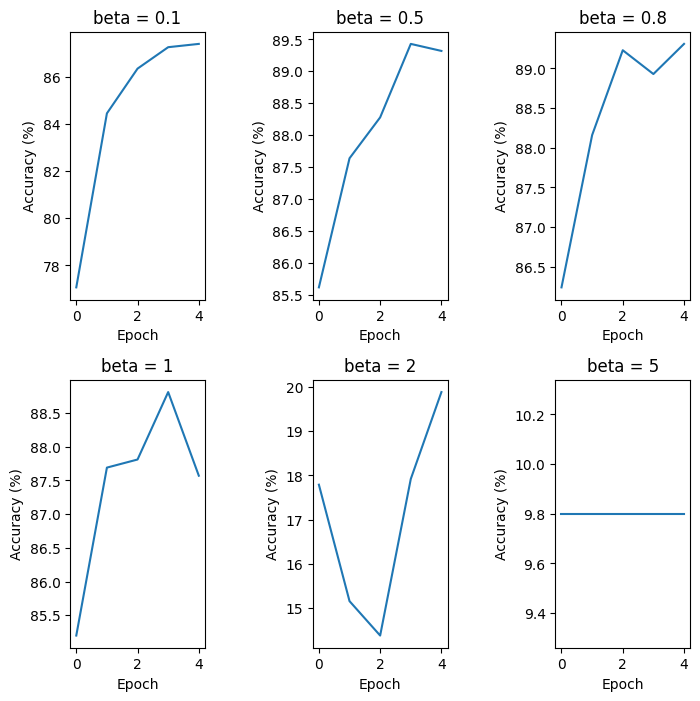
\includegraphics[width=0.75\textwidth]{beta_tuning.png}
    \caption{Tuning $\beta$ hyperparameter}
    \label{fig:beta_tuning}
\end{figure}
From the graphs of test accuracy with increasing $\beta$ values in Figure \ref{fig:beta_tuning} we can see that the performance steadily improves up to $\beta = 0.1$ and then starts to decrease. At $\beta = 2$ the accuracy is starts below 18\% and additional training epochs increases it up to 20\%. At $beta = 5$ the accuracy stays at exactly 9.8\%. We can most likely attribute this behavior due to large $\beta$ values weighting previous membrane potentials much higher than the threshold potential. \[
    V_{t+1} = \beta V_t + I_t - o_{t+1} \cdot V_{th}
\]
The above equation describes the relationship between the current membrane potential and the membrane potential at the next timestep. If $\beta$ is large, the previous membrane potential $V_t$ will have a large effect on the current membrane potential $V_{t+1}$ and if $V_{th}$ is small, the neuron will always fire leading to about a 10\% accuracy.

\begin{figure}[H]
    \centering
    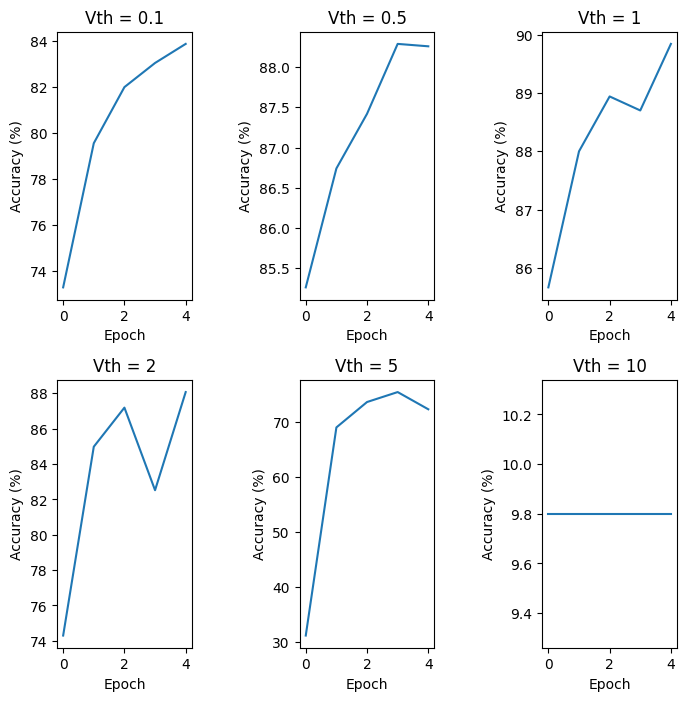
\includegraphics[width=0.75\textwidth]{vth_tuning.png}
    \caption{Tuning $V_{th}$ hyperparameter}
    \label{fig:vth_tuning}
\end{figure}
The test accuracies for different $V_{th}$ values in Figure \ref{fig:vth_tuning} shows a similar trend to the previous hyperparameter tuning results. Performance steadily improves up to $V_{th} = 1$ and then starts to decrease. At $V_{th} = 5$ the accuracy levels out below 80\%. This could be attributed to the fact that the threshold potential is too high for the neuron to fire. If the threshold potential is too high, the neuron will not fire and the network will not learn. At $V_{th} = 10$ the accuracy is at 10\% and additional training epochs does not show any improvement in the accuracy. This could be attributed to the fact that the threshold potential is too high for the neuron to fire. If the threshold potential is too high, the neuron will never fire and the prediction would just be a random guess.

\begin{figure}[H]
    \centering
    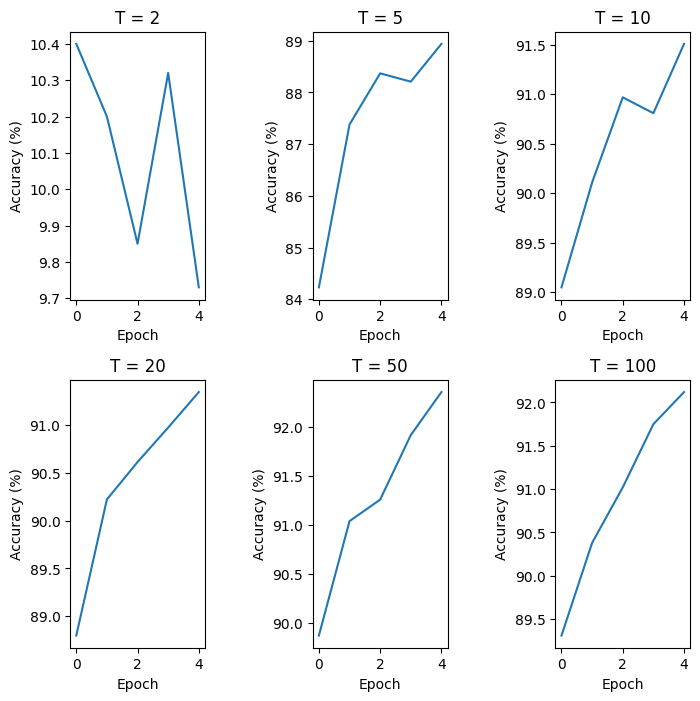
\includegraphics[width=0.75\textwidth]{t_tuning.png}
    \caption{Tuning $T$ hyperparameter}
    \label{fig:v_tuning}
\end{figure}
The test accuracies for different $T$ values in Figure \ref{fig:v_tuning} shows a slightly different trend. At $T=2$ The accuracy was below 10\% and decreased over training epochs. This could be attributed to not having enough steps to build up membrane potential for the neurons to fire. $T = 50$ had the highest test accuracy after training ending at 93\%. At higher $T$ the input data is duplicated more times which could allow the network to better fit to the training data leading to higher accuracy. At $T = 100$ though the accuracy peaks at 92\% which is slightly lower than $T = 50$. Following a similar train of thought this might be due to overfitting the training data since we are duplicating the input data 100 times. Something else to note is that the training time as $T$ increases also increases. This is due to the fact that in the forward pass we are looping through the input data $T$ times.

\setcounter{subsubsection}{4}
\subsubsection{Different ways of generating input data}
While the MNIST input data for ANNs is just a batch of ${H \times W}$ images that we can flatten before feeding it into the network for SNNs we need to convert each image to a time sequence of inputs. There are multiple ways to do this in one case we can simply duplicate the input data $T$ times and feed it into the network. Another way to generate input data is to use a threshold value where if the pixel value is greater than the threshold we keep it the same otherwise set it to be 0. The final way is to treat each pixel as a bernoulli random variable with mean defined by the pixel intensity. At each timestep we sample from the pixel bernoulli variables to determine the image at the timestep. Below are the test accuracies for the different ways of generating input data.

\begin{figure}[H]
    \centering
    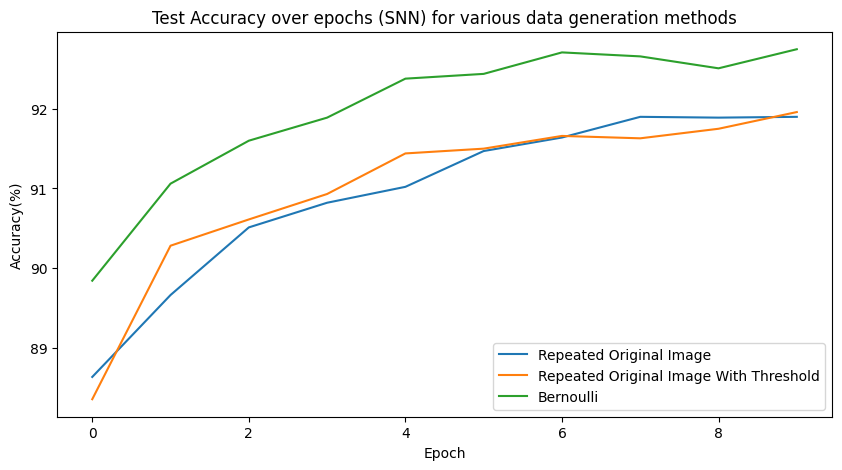
\includegraphics[width=1\textwidth]{data_gen.png}
    \caption{Comparing data generation methods}
    \label{fig:data_gen}
\end{figure}

We can see from the test accuracy results the Bernoulli random sampling method of generating the input at each timestep has a significantly higher accuracy compared to the other two methods. This is probably because using random sampling we can introduce more sparsity to the input data which is beneficial for SNNs. 

\subsection{Different Loss Functions}
For the above training we used the mean squared error loss function to achieve a maximum test accuracy of 93\%. Traditionally, MSE loss is better suited for regression tasks where expected values are continuous but in the MNIST classification task outputs are discrete. In theory we can also use the cross entropy loss function for training the network which should perform better than MSE. Below are the test accuracies for the different loss functions.

\begin{figure}[H]
    \centering
    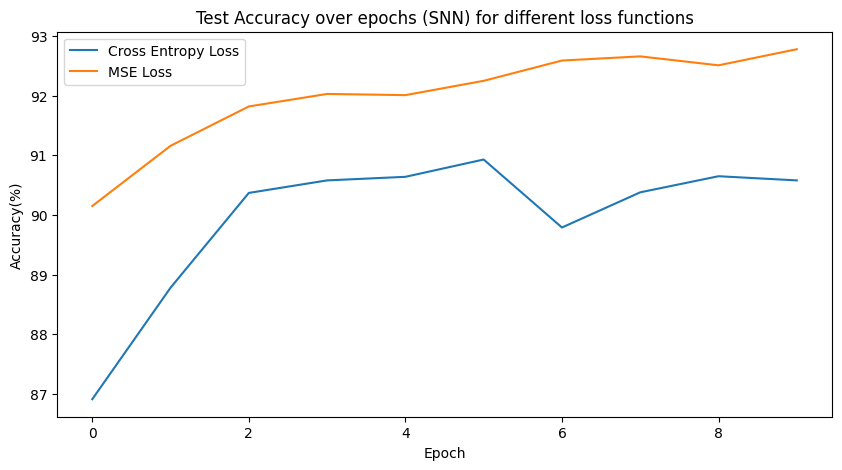
\includegraphics[width=1\textwidth]{loss_functions.png}
    \caption{Comparing loss functions}
    \label{fig:loss_functions}
\end{figure}

From the test accuracy results suprisingly the MSE loss function performed better than the cross entropy loss function. One possible explanation is that because the outputs are a firing rate which is normalized based on the number of timesteps, cross entropy loss might not be penalizing incorrect predictions or encouraging correct predictions as much as MSE loss. Looking at the graph for $e^{x}$ x values that are below 1 have generally a smaller gradient which could be a reason why the network is not learning as well as with MSE loss.

\subsection{FLOPs Calculation}
The FLOPs calculation formula for a single fully connected layer in an ANN is \[
    FLOPs = (2 \cdot M - 1) \cdot N + 2N
\] while the FLOPs calculation formula for a single fully connected layer in an SNN for a single timestep is \[
    FLOPs = (2 \cdot M \cdot F - 1) \cdot N + 2N
\] where $M$ is the input size, $N$ is the output size, and $F$ is the average firing rate of the previous layer. For the MNIST dataset one forward pass FLOPs for an ANN is straightforward. The first layer has 784 input nodes and 10 output nodes, the second layer has 10 input nodes and 10 output nodes so the total FLOPs for one forward pass is \[
    FLOPs = (2 \cdot 784 - 1) \cdot 10 + 2 \cdot 10 + (2 \cdot 10 - 1) \cdot 10 + 2 \cdot 10 = 15900
\] Since this value doesn't vary between batches the average ANN FLOPs is also $15900$. For SNN we need to calculate the average firing rate of the previous layer at each timestep during training and validation. For the first fully connected layer since the input was generated using a bernoulli random variable that means each pixel value is a 0 or 1. We can treat a 1 as a spike and a 0 as no spike. The average firing rate would be the sum of all values in each input of the batch divided by 784 and then averaged across all batches. The formula looks like \[
    F = \frac{1}{B} \sum_{b=1}^{B} \frac{1}{M} \sum_{i=1}^{M} x_{b,i}
\] where $B$ is the number of batches, where $M$ is the input size, $b$ is the batch index, $x_{b,i}$ is the pixel value at index $i$ in batch $b$. We can use the same formula for computing the average firing rate for the second fully connected layer. Using the firing rates we can now compute a single timesteps FLOPs but for one forward pass we have $T$ timesteps so we need to add all $T$ timesteps FLOPs to get the total FLOPs for one forward pass. Given the FLOPs for one forward pass we can then average across all batches to get an average FLOPs for one forward pass for a single epoch. The graph below shows the average FLOPs over epochs for training and validation.

\begin{figure}[H]
    \centering
    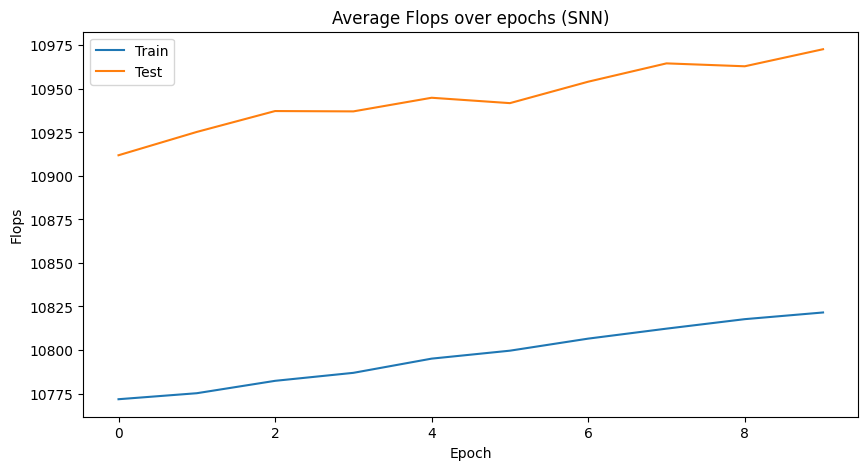
\includegraphics[width=1\textwidth]{flops_snn.png}
    \caption{Comparing data generation methods}
    \label{fig:flops_snn}
\end{figure}

We can see that the average FLOPs for validation are higher than that for training and they both steadily increase over the epochs. We can take the average across all epochs and then compare that to the average we have for ANNs. The average ANN FLOPs is $15900$ from above and the average SNN FLOPs where $T = 5$ for the validation set is $10945$. There was about a 31\% reduction in FLOPs for the SNN compared to the ANN. This is because the SNN is able to take advantage of the sparsity of the input data and only make computations when there is a spike.

\end{document}